% Brief expl
This appendix reports all graphs and tables related to all the writing experiments conducted. Results are reported first expressed as latency (measured during the experiments), then as throughput (computed from the latency and table size).

%%%%%%%%%%%%%%%%%%%%%%%%%%%%%%%%%%%%%%%%%%%%%%%%%%%%%%%%%%%%%%%%%
%%%%%%%%%%%%              LATENCY             %%%%%%%%%%%%%%%%%%%
%%%%%%%%%%%%%%%%%%%%%%%%%%%%%%%%%%%%%%%%%%%%%%%%%%%%%%%%%%%%%%%%%
\begin{figure}
    \centering
    \begin{minipage}[b]{\textwidth}
        \centering
        \captionof{table}[Write experiment - Latency - 1 CPU core]{Write experiment results expressed as latency. The experiment was performed with one \glstext{CPU} core.}
        \label{tbl:appx_res_write_time_1_core}
        \begin{tabular}{c r S[table-format=5.5] S[table-format=5.5] S[table-format=5.5]} 
            \toprule
            \multirow{2}{*}{{Pipeline\Tstrut\Bstrut}} & \multirow{2}{*}{{\thead{Number\\ of rows}}} & {\multirow{2}{*}{{\thead{Latency \\ (seconds)}}}} & \multicolumn{2}{c}{{\thead{Latency (seconds) \\95\% Confidence Interval}}}\\
                                                      &                                             &                                                   & {low} & {high}\\
            \midrule
            \multirow{5}{4em}{delta-rs\\ HopsFS} & 10K  &    1.25088 &    1.23807 &   1.26545\\ 
                                                 & 100K &    1.36828 &    1.33757 &   1.38982\\ 
                                                 & 1M   &    9.38152 &    9.23971 &   9.52904\\
                                                 & 6M   &   19.75469 &   19.33270 &  20.11785\\
                                                 & 60M  &  177.30707 &  174.62871 & 180.01732\\
            \midrule
            \multirow{5}{4em}{delta-rs\\ LocalFS} & 10K  &    0.03957 &   0.03770 &   0.04153\\ 
                                                  & 100K &    0.15240 &   0.14598 &   0.15888\\ 
                                                  & 1M   &    8.42252 &   8.28396 &   8.56376\\
                                                  & 6M   &   17.90634 &  17.48040 &  18.33585\\
                                                  & 60M  &  172.34552 & 169.74808 & 174.73138\\
            \midrule
            \multirow{5}{4em}{Legacy} & 10K  &    50.22767 &   49.53501 &   50.93664\\ 
                                      & 100K &    59.56187 &   58.89466 &   60.18496\\ 
                                      & 1M   &   112.19048 &  111.37162 &  113.00915\\
                                      & 6M   &   511.81693 &  510.75113 &  512.83672\\
                                      & 60M  &  2715.77285 & 2699.88061 & 2731.95225\\
            \bottomrule
        \end{tabular}
    \end{minipage}
    \begin{minipage}[b]{\textwidth}
        \centering
        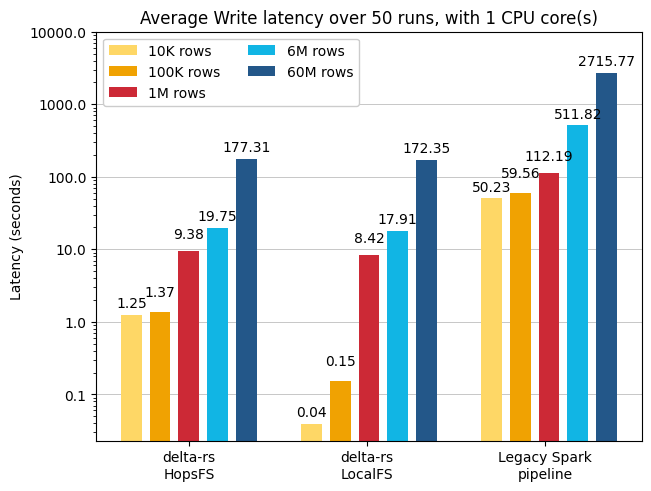
\includegraphics[width=\textwidth]{figures/99-appendix/results-diagrams/write/write_time_1_core.png}
        \caption[Histogram of the write experiment - Latency - 1 CPU core]{Histogram in log-scale of the write experiment results expressed as latency. The experiment was performed with one \glstext{CPU} core.}
        \label{fig:appx_res_write_time_1_core}
    \end{minipage}
\end{figure}

\begin{figure}
    \centering
    \begin{minipage}[b]{\textwidth}
        \centering
        \captionof{table}[Write experiment - Latency - 2 CPU cores]{Write experiment results expressed as latency. The experiment was performed with two \glstext{CPU} cores.}
        \label{tbl:appx_res_write_time_2_cores}
        \begin{tabular}{c r S[table-format=5.5] S[table-format=5.5] S[table-format=5.5]} 
            \toprule
            \multirow{2}{*}{{Pipeline\Tstrut\Bstrut}} & \multirow{2}{*}{{\thead{Number\\ of rows}}} & {\multirow{2}{*}{{\thead{Latency \\ (seconds)}}}} & \multicolumn{2}{c}{{\thead{Latency (seconds) \\95\% Confidence Interval}}}\\
                                                      &                                             &                                                   & {low} & {high}\\
            \midrule
            \multirow{5}{4em}{delta-rs\\ HopsFS} & 10K  &    1.26239 &    1.25079 &   1.27639\\ 
                                                 & 100K &    1.30812 &    1.28050 &   1.33217\\ 
                                                 & 1M   &    8.51536 &    8.34333 &   8.70077\\
                                                 & 6M   &   16.29042 &   15.90659 &  16.67362\\
                                                 & 60M  &  134.06089 &  131.65031 & 136.39761\\
            \midrule
            \multirow{5}{4em}{delta-rs\\ LocalFS} & 10K  &    0.04823 &   0.04640 &   0.04997\\ 
                                                  & 100K &    0.13714 &   0.13402 &   0.14050\\ 
                                                  & 1M   &    7.18530 &   7.03747 &   7.35128\\
                                                  & 6M   &   15.26632 &  14.85172 &  15.65167\\
                                                  & 60M  &  129.82007 & 127.60020 & 132.04689\\
            \midrule
            \multirow{5}{4em}{Legacy} & 10K  &    50.72405 &   50.10769 &   51.30686\\ 
                                      & 100K &    59.78810 &   58.97997 &   60.47427\\ 
                                      & 1M   &   108.56499 &  108.01124 &  109.08128\\
                                      & 6M   &   473.37954 &  472.34534 &  474.43740\\
                                      & 60M  &  2340.77013 & 2333.99443 & 2347.97127\\
            \bottomrule
        \end{tabular}
    \end{minipage}
    \begin{minipage}[b]{\textwidth}
        \centering
        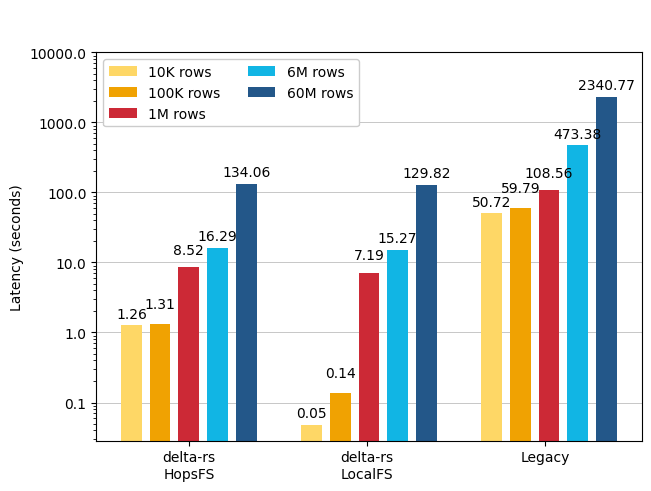
\includegraphics[width=\textwidth]{figures/99-appendix/results-diagrams/write/write_time_2_core.png}
        \caption[Histogram of the write experiment - Latency - 2 CPU cores]{Histogram in log-scale of the write experiment results expressed as latency. The experiment was performed with two \glstext{CPU} cores.}
        \label{fig:appx_res_write_time_2_cores}
    \end{minipage}
\end{figure}

\begin{figure}
    \centering
    \begin{minipage}[b]{\textwidth}
        \centering
        \captionof{table}[Write experiment - Latency - 4 CPU cores]{Write experiment results expressed as latency. The experiment was performed with four \glstext{CPU} cores.}
        \label{tbl:appx_res_write_time_4_cores}
        \begin{tabular}{c r S[table-format=5.5] S[table-format=5.5] S[table-format=5.5]} 
            \toprule
            \multirow{2}{*}{{Pipeline\Tstrut\Bstrut}} & \multirow{2}{*}{{\thead{Number\\ of rows}}} & {\multirow{2}{*}{{\thead{Latency \\ (seconds)}}}} & \multicolumn{2}{c}{{\thead{Latency (seconds) \\95\% Confidence Interval}}}\\
                                                      &                                             &                                                   & {low} & {high}\\
            \midrule
            \multirow{5}{4em}{delta-rs\\ HopsFS} & 10K  &    1.21642 &    1.20232 &   1.23231\\ 
                                                 & 100K &    1.33622 &    1.32294 &   1.34942\\ 
                                                 & 1M   &    8.41325 &    8.24770 &   8.58272\\
                                                 & 6M   &   16.22402 &   15.87946 &  16.59586\\
                                                 & 60M  &  124.10242 &  121.57723 & 126.81530\\
            \midrule
            \multirow{5}{4em}{delta-rs\\ LocalFS} & 10K  &    0.04572 &   0.04341 &   0.04807\\ 
                                                  & 100K &    0.13176 &   0.12880 &   0.13499\\ 
                                                  & 1M   &    7.18574 &   7.00679 &   7.36343\\
                                                  & 6M   &   14.55578 &  14.17679 &  14.94192\\
                                                  & 60M  &  121.37623 & 119.17256 & 123.69890\\
            \midrule
            \multirow{5}{4em}{Legacy} & 10K  &    51.28465 &   50.62282 &   51.90367\\ 
                                      & 100K &    59.52655 &   58.90537 &   60.15322\\ 
                                      & 1M   &   108.81674 &  108.25217 &  109.34234\\
                                      & 6M   &   481.98353 &  481.04435 &  482.92992\\
                                      & 60M  &  2346.04687 & 2336.99396 & 2355.19897\\
            \bottomrule
        \end{tabular}
    \end{minipage}
    \begin{minipage}[b]{\textwidth}
        \centering
        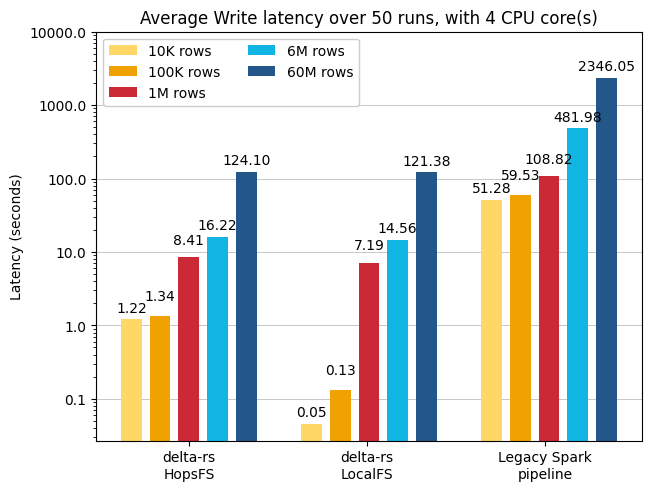
\includegraphics[width=\textwidth]{figures/99-appendix/results-diagrams/write/write_time_4_core.png}
        \caption[Histogram of the write experiment - Latency - 4 CPU cores]{Histogram in log-scale of the write experiment results expressed as latency. The experiment was performed with four \glstext{CPU} cores.}
        \label{fig:appx_res_write_time_4_cores}
    \end{minipage}
\end{figure}

\begin{figure}
    \centering
    \begin{minipage}[b]{\textwidth}
        \centering
        \captionof{table}[Write experiment - Latency - 8 CPU cores]{Write experiment results expressed as latency. The experiment was performed with eight \glstext{CPU} cores.}
        \label{tbl:appx_res_write_time_8_cores}
        \begin{tabular}{c r S[table-format=5.5] S[table-format=5.5] S[table-format=5.5]} 
            \toprule
            \multirow{2}{*}{{Pipeline\Tstrut\Bstrut}} & \multirow{2}{*}{{\thead{Number\\ of rows}}} & {\multirow{2}{*}{{\thead{Latency \\ (seconds)}}}} & \multicolumn{2}{c}{{\thead{Latency (seconds) \\95\% Confidence Interval}}}\\
                                                      &                                             &                                                   & {low} & {high}\\
            \midrule
            \multirow{5}{4em}{delta-rs\\ HopsFS} & 10K  &    1.36756 &    1.24934 &   1.57224\\ 
                                                 & 100K &    1.29243 &    1.26548 &   1.31099\\ 
                                                 & 1M   &    8.30120 &    8.14918 &   8.47040\\
                                                 & 6M   &   15.73847 &   15.28974 &  16.16084\\
                                                 & 60M  &  121.95014 &  119.59376 & 124.18097\\
            \midrule
            \multirow{5}{4em}{delta-rs\\ LocalFS} & 10K  &    0.04402 &   0.04174 &   0.04640\\ 
                                                  & 100K &    0.13648 &   0.13281 &   0.14061\\ 
                                                  & 1M   &    7.22872 &   7.07511 &   7.39893\\
                                                  & 6M   &   14.28157 &  13.90508 &  14.66126\\
                                                  & 60M  &  119.97915 & 117.76416 & 122.20882\\
            \midrule
            \multirow{5}{4em}{Legacy} & 10K  &    51.22859 &   50.59478 &   51.86476\\ 
                                      & 100K &    60.27751 &   59.72907 &   60.77130\\ 
                                      & 1M   &   109.38189 &  108.86830 &  109.88263\\
                                      & 6M   &   475.94345 &  474.83993 &  477.05274\\
                                      & 60M  &  2324.97917 & 2319.04203 & 2331.04794\\
            \bottomrule
        \end{tabular}
    \end{minipage}
    \begin{minipage}[b]{\textwidth}
        \centering
        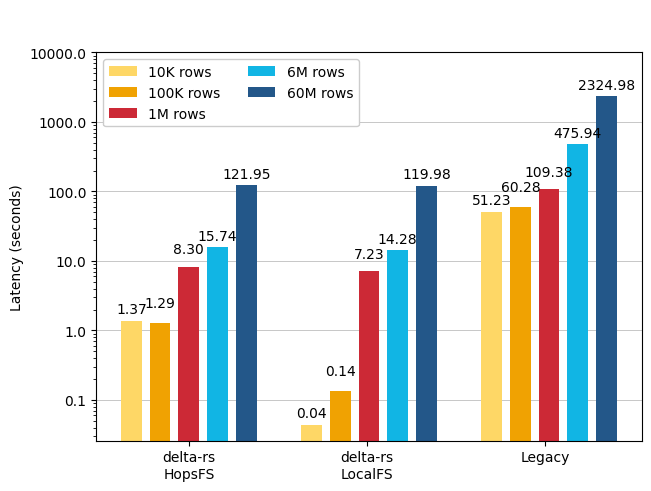
\includegraphics[width=\textwidth]{figures/99-appendix/results-diagrams/write/write_time_8_core.png}
        \caption[Histogram of the write experiment - Latency - 8 CPU cores]{Histogram in log-scale of the write experiment results expressed as latency. The experiment was performed with eight \glstext{CPU} cores.}
        \label{fig:appx_res_write_time_8_cores}
    \end{minipage}
\end{figure}

%%%%%%%%%%%%%%%%%%%%%%%%%%%%%%%%%%%%%%%%%%%%%%%%%%%%%%%%%%%%%%%%%
%%%%%%%%%%%%             THROUGHPUT           %%%%%%%%%%%%%%%%%%%
%%%%%%%%%%%%%%%%%%%%%%%%%%%%%%%%%%%%%%%%%%%%%%%%%%%%%%%%%%%%%%%%%

\begin{figure}
    \centering
    \begin{minipage}[b]{\textwidth}
        \centering
        \captionof{table}[Write experiment - Throughput - 1 CPU core]{Write experiment results expressed as throughput. The experiment was performed with one \glstext{CPU} core.}
        \label{tbl:appx_res_write_throughput_1_core}
        \begin{tabular}{c r S[table-format=5.5] S[table-format=5.5] S[table-format=5.5]} 
            \toprule
            \multirow{2}{*}{{Pipeline\Tstrut\Bstrut}} & \multirow{2}{*}{{\thead{Number\\ of rows}}} & {\multirow{2}{*}{{\thead{Throughput \\ (k rows/second)}}}} & \multicolumn{2}{c}{{\thead{Throughput (k rows/second) \\95\% Confidence Interval}}}\\
                                                      &                                             &                                                          & {low} & {high}\\
            \midrule
            \multirow{5}{4em}{delta-rs\\ HopsFS} & 10K  &    7.99436 &    7.90230 &   8.07705\\ 
                                                 & 100K &    7.30843 &    7.19514 &   7.47621\\ 
                                                 & 1M   &  106.59242 &  104.94226 & 108.22850\\
                                                 & 6M   &  303.72533 &  298.24252 & 310.35491\\
                                                 & 60M  &  338.39598 &  333.30126 & 343.58610\\
            \midrule
            \multirow{5}{4em}{delta-rs\\ LocalFS} & 10K  &  252.68238 &  240.73405 &  265.18632\\ 
                                                  & 100K &  656.15739 &  629.36777 &  684.98518\\ 
                                                  & 1M   &  118.72919 &  116.77110 &  120.71514\\
                                                  & 6M   &  335.07675 &  327.22770 &  343.24143\\
                                                  & 60M  &  348.13784 &  343.38422 &  353.46496\\
            \midrule
            \multirow{5}{4em}{Legacy} & 10K  &     0.19909 &    0.19632 &    0.20187\\ 
                                      & 100K &     1.67892 &    1.66154 &    1.69794\\ 
                                      & 1M   &     8.91341 &    8.84884 &    8.97894\\
                                      & 6M   &    11.72294 &   11.69963 &   11.74740\\
                                      & 60M  &    22.09315 &   21.96231 &   22.22320\\
            \bottomrule
        \end{tabular}
    \end{minipage}
    \begin{minipage}[b]{\textwidth}
        \centering
        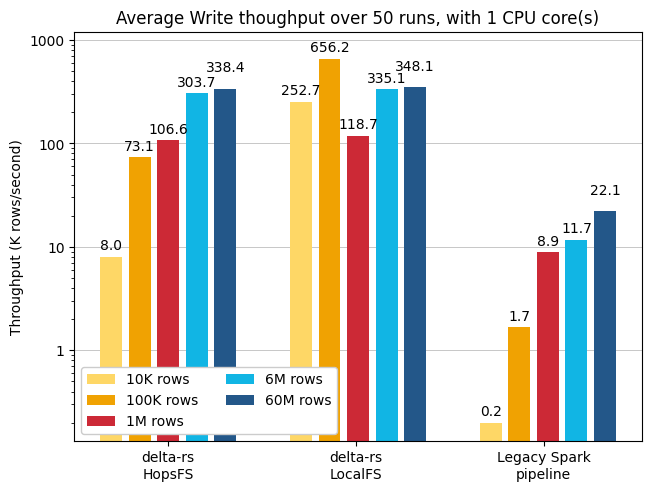
\includegraphics[width=\textwidth]{figures/99-appendix/results-diagrams/write/write_throughput_1_core.png}
        \caption[Histogram of the write experiment - Throughput - 1 CPU core]{Histogram in log-scale of the write experiment results expressed as throughput. The experiment was performed with one \glstext{CPU} core.}
        \label{fig:appx_res_write_throughput_1_core}
    \end{minipage}
\end{figure}

\begin{figure}
    \centering
    \begin{minipage}[b]{\textwidth}
        \centering
        \captionof{table}[Write experiment - Throughput - 2 CPU cores]{Write experiment results expressed as throughput. The experiment was performed with two \glstext{CPU} cores.}
        \label{tbl:appx_res_write_throughput_2_cores}
        \begin{tabular}{c r S[table-format=5.5] S[table-format=5.5] S[table-format=5.5]} 
            \toprule
            \multirow{2}{*}{{Pipeline\Tstrut\Bstrut}} & \multirow{2}{*}{{\thead{Number\\ of rows}}} & {\multirow{2}{*}{{\thead{Throughput \\ (k rows/second)}}}} & \multicolumn{2}{c}{{\thead{Throughput (k rows/second) \\95\% Confidence Interval}}}\\
                                                      &                                             &                                                          & {low} & {high}\\
            \midrule
            \multirow{5}{4em}{delta-rs\\ HopsFS} & 10K  &    7.92146 &    7.83458 &   7.99491\\ 
                                                 & 100K &   76.44507 &   75.06499 &  78.09433\\ 
                                                 & 1M   &  117.43478 &  114.93231 & 119.85614\\
                                                 & 6M   &  368.31440 &  359.84975 & 377.20198\\
                                                 & 60M  &  447.55780 &  439.89038 & 455.75281\\
            \midrule
            \multirow{5}{4em}{delta-rs\\ LocalFS} & 10K  &  207.31922 &  200.08626 &  215.49342\\ 
                                                  & 100K &  729.15967 &  711.73966 &  746.13854\\ 
                                                  & 1M   &  139.17297 &  136.03055 &  142.09647\\
                                                  & 6M   &  393.02185 &  383.34560 &  403.99352\\
                                                  & 60M  &  462.17814 &  454.38403 &  470.21868\\
            \midrule
            \multirow{5}{4em}{Legacy} & 10K  &     0.19714 &    0.19490 &    0.19957\\ 
                                      & 100K &     1.67257 &    1.65359 &    1.69549\\ 
                                      & 1M   &     9.21107 &    9.16747 &    9.25829\\
                                      & 6M   &    12.67481 &   12.64655 &   12.70257\\
                                      & 60M  &    25.63258 &   25.55397 &   25.70700\\
            \bottomrule
        \end{tabular}
    \end{minipage}
    \begin{minipage}[b]{\textwidth}
        \centering
        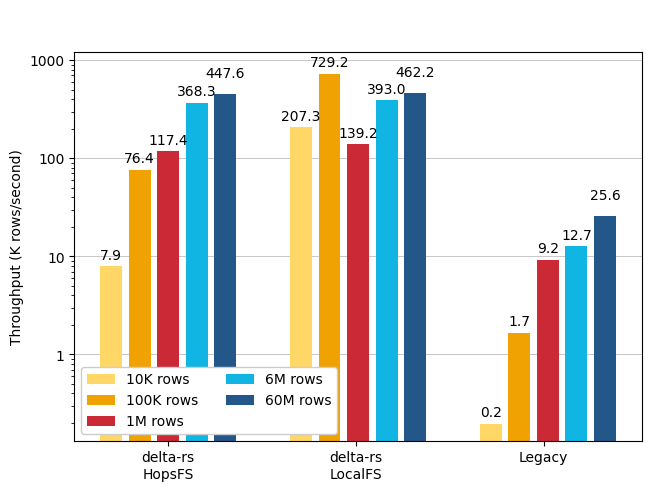
\includegraphics[width=\textwidth]{figures/99-appendix/results-diagrams/write/write_throughput_2_core.png}
        \caption[Histogram of the write experiment - Throughput - 2 CPU cores]{Histogram in log-scale of the write experiment results expressed as throughput. The experiment was performed with two \glstext{CPU} cores.}
        \label{fig:appx_res_write_throughput_2_cores}
    \end{minipage}
\end{figure}

\begin{figure}
    \centering
    \begin{minipage}[b]{\textwidth}
        \centering
        \captionof{table}[Write experiment - Throughput - 4 CPU cores]{Write experiment results expressed as throughput. The experiment was performed with four \glstext{CPU} cores.}
        \label{tbl:appx_res_write_throughput_4_cores}
        \begin{tabular}{c r S[table-format=5.5] S[table-format=5.5] S[table-format=5.5]} 
            \toprule
            \multirow{2}{*}{{Pipeline\Tstrut\Bstrut}} & \multirow{2}{*}{{\thead{Number\\ of rows}}} & {\multirow{2}{*}{{\thead{Throughput \\ (k rows/second)}}}} & \multicolumn{2}{c}{{\thead{Throughput (k rows/second) \\95\% Confidence Interval}}}\\
                                                      &                                             &                                                          & {low} & {high}\\
            \midrule
            \multirow{5}{4em}{delta-rs\\ HopsFS} & 10K  &    8.22083 &    8.11482 &   8.11482\\ 
                                                 & 100K &   74.83742 &   74.10566 &  75.58871\\ 
                                                 & 1M   &  118.86008 &  116.51310 & 121.24582\\
                                                 & 6M   &  369.82202 &  361.53577 & 377.84652\\
                                                 & 60M  &  483.47160 &  473.12899 & 493.51343\\
            \midrule
            \multirow{5}{4em}{delta-rs\\ LocalFS} & 10K  &  218.71364 &  208.02604 &  230.31412\\ 
                                                  & 100K &  758.92422 &  740.79474 &  776.39115\\ 
                                                  & 1M   &  139.16432 &  135.80613 &  142.71864\\
                                                  & 6M   &  412.20728 &  401.55459 &  423.22678\\
                                                  & 60M  &  494.33070 &  485.04875 &  503.47156\\
            \midrule
            \multirow{5}{4em}{Legacy} & 10K  &     0.19499 &    0.19266 &    0.19753\\ 
                                      & 100K &     1.67992 &    1.66242 &    1.69763\\ 
                                      & 1M   &     9.18976 &    9.14558 &    9.23768\\
                                      & 6M   &    12.44855 &   12.42416 &   12.47286\\
                                      & 60M  &    25.57493 &   25.47555 &   25.67400\\
            \bottomrule
        \end{tabular}
    \end{minipage}
    \begin{minipage}[b]{\textwidth}
        \centering
        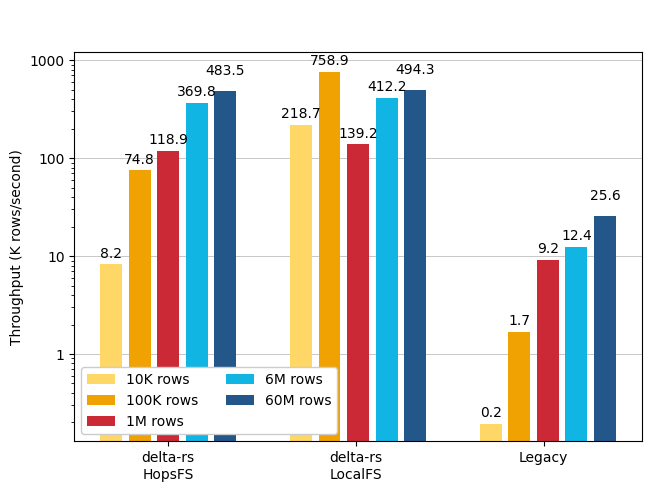
\includegraphics[width=\textwidth]{figures/99-appendix/results-diagrams/write/write_throughput_4_core.png}
        \caption[Histogram of the write experiment - Throughput - 4 CPU cores]{Histogram in log-scale of the write experiment results expressed as throughput. The experiment was performed with four \glstext{CPU} cores.}
        \label{fig:appx_res_write_throughput_4_cores}
    \end{minipage}
\end{figure}

\begin{figure}
    \centering
    \begin{minipage}[b]{\textwidth}
        \centering
        \captionof{table}[Write experiment - Throughput - 8 CPU cores]{Write experiment results expressed as throughput. The experiment was performed with eight \glstext{CPU} cores.}
        \label{tbl:appx_res_write_throughput_8_cores}
        \begin{tabular}{c r S[table-format=5.5] S[table-format=5.5] S[table-format=5.5]} 
            \toprule
            \multirow{2}{*}{{Pipeline\Tstrut\Bstrut}} & \multirow{2}{*}{{\thead{Number\\ of rows}}} & {\multirow{2}{*}{{\thead{Throughput \\ (k rows/second)}}}} & \multicolumn{2}{c}{{\thead{Throughput (k rows/second) \\95\% Confidence Interval}}}\\
                                                      &                                             &                                                          & {low} & {high}\\
            \midrule
            \multirow{5}{4em}{delta-rs\\ HopsFS} & 10K  &    7.31228 &    6.36032 &    8.00422\\ 
                                                 & 100K &   77.37337 &   76.27782 &   79.02104\\ 
                                                 & 1M   &  120.46439 &  118.05814 &  122.71160\\
                                                 & 6M   &  381.23126 &  371.26772 &  392.41978\\
                                                 & 60M  &  492.00431 &  483.16579 &  501.69837\\
            \midrule
            \multirow{5}{4em}{delta-rs\\ LocalFS} & 10K  &  227.12095 &  215.48714 &  239.54128\\ 
                                                  & 100K &  732.70141 &  711.16038 &  752.93200\\ 
                                                  & 1M   &  138.33701 &  135.15466 &  141.34041\\
                                                  & 6M   &  420.12165 &  409.24176 &  431.49669\\
                                                  & 60M  &  500.08688 &  490.96288 &  509.49286\\
            \midrule
            \multirow{5}{4em}{Legacy} & 10K  &     0.19520 &    0.19280 &    0.19764\\ 
                                      & 100K &     1.65899 &    1.64551 &    1.67422\\ 
                                      & 1M   &     9.14228 &    9.10061 &    9.18540\\
                                      & 6M   &    12.60653 &   12.57722 &   12.63583\\
                                      & 60M  &    25.80668 &   25.73949 &   25.87275\\
            \bottomrule
        \end{tabular}
    \end{minipage}
    \begin{minipage}[b]{\textwidth}
        \centering
        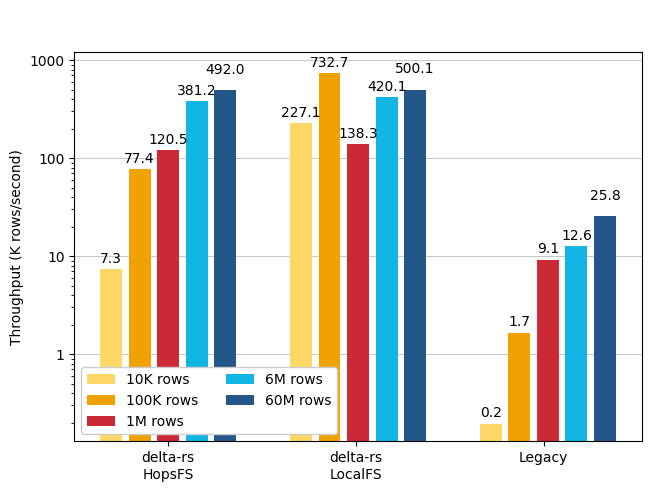
\includegraphics[width=\textwidth]{figures/99-appendix/results-diagrams/write/write_throughput_8_core.png}
        \caption[Histogram of the write experiment - Throughput - 8 CPU cores]{Histogram in log-scale of the write experiment results expressed as throughput. The experiment was performed with eight \glstext{CPU} cores.}
        \label{fig:appx_res_write_throughput_8_cores}
    \end{minipage}
\end{figure}